\documentclass[10pt]{article}
\usepackage[utf8]{inputenc}
\usepackage{array, xcolor, bibentry}
\usepackage[margin=3cm]{geometry}

\usepackage[spanish]{babel}
\selectlanguage{spanish}

\usepackage{graphicx}
\graphicspath{ {./img/} }

\title{\bfseries M. Joaquín García González}
\author{info@manliogarcia.es}
\date{}

\definecolor{lightgray}{gray}{0.8}
\newcolumntype{L}{>{\raggedleft}p{0.18\textwidth}}
\newcolumntype{R}{p{0.8\textwidth}}
\newcommand\VRule{\color{lightgray}\vrule width 0.5pt}

\begin{document}
    \pagenumbering{gobble}% Remove page numbers (and reset to 1)

    \maketitle

    \begin{minipage}[ht]{0.48\textwidth}
        Urb. Porlier, Módulo ``o'', Nº 8\\
        C/ General, Bajamar 38250\\
        San Cristóbal de La Laguna\\
        \\
        Nacionalidad: Español, Argentino\\
        Fecha de nacimiento: 29 de Octubre de 1990\\
        Teléfono de contacto: +34 655 141 227
    \end{minipage}
    \begin{minipage}[ht]{0.48\textwidth}
        \begin{flushright}
        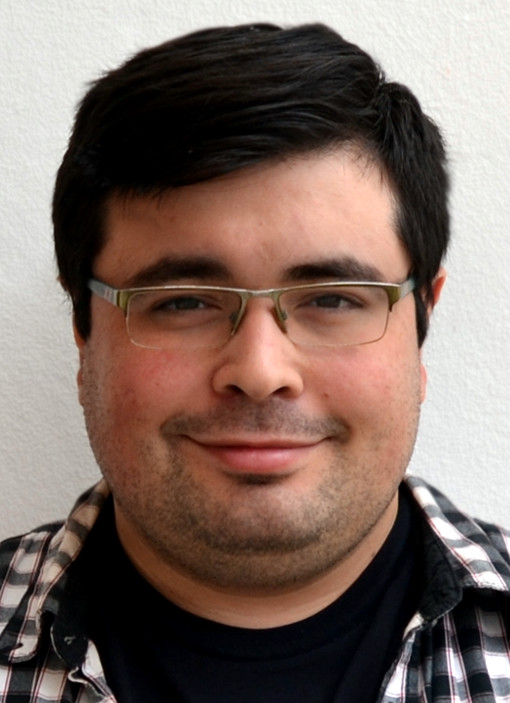
\includegraphics[height=8em]{profile}
        \end{flushright}
    \end{minipage}

    \section*{Lenguajes de programación}
    \begin{center}
    \begin{tabular}{ c c c c c c c c c c c c }

      Bash & Elixir & Ruby & Python & Javascript & CSS \\\\

         Golang & Java & C\# & PHP & Unity-Script & \LaTeX

    \end{tabular}
    \end{center}

    \section*{Idiomas}
    \begin{tabular}{L!{\VRule}R}

        Español&Lengua materna\\\\

        Inglés&Fluido (Certificado B2 por la escuela oficial de idiomas de La Laguna en 2009.)\\\\

    \end{tabular}

    \section*{Experiencia Profesional}
    \begin{tabular}{L!{\VRule}R}

        2016--Actualidad&{{\bf Administración de sistemas y desarrollo
        independiente.}\newline Mi trabajo como desarrollador freelance
        consiste en el desarrollo de soluciones digitales a medida y páginas
        web corporativas para nuestros clientes. También realizo administración
        de los servidores, así como mejoras técnicas a la infraestructura
        cuando no estoy en un proyecto.}\\\\

        2019&{Desarrollador DevOps en Aresoltec Canarias S.L.}\\\\

        2018--2019&{Desarrollador DevOps en Canarias Infopista S.L.}\\\\

        2015--2016&{Administración del aula de informática bajo la supervisión
        de la Oficina de Software Libre para la Universidad de La Laguna.}\\\\

        2015--2016&{Servicio técnico para la empresa Horizont Atlantic SL.}\\\\

        2011--2014&{Desarrollo de videojuegos para la empresa 4D3 Studio.}\\\\

        2014&{Diseño de videojuego para móviles geolocalizado ``Progrezz''}\\\\

    \end{tabular}

    \section*{Experiencia Profesional}
    \begin{tabular}{L!{\VRule}R}

        2014&Miembro colaborador en la organización y maquetación del ``XV
        Congreso Internacional de Interacción Persona Ordenador 2014'',
        celebrada en el
        Puerto de la Cruz en septiembre de 2014.\\\\

        2011--2012&{Colaboración en el desarrollo del videojuego Mundo Isla
        para la Universidad de La Laguna en el proyecto para la promoción de
        los hábitos saludables ``SAVEH''}.\\\\

        2009--2012&{Cartelería para títulos propios de la Universidad de La
        Laguna.}\\\\

    \end{tabular}

    \section*{Voluntariado y Software Libre}
    \begin{tabular}{L!{\VRule}R}

        2009&{Voluntario técnico en el evento de software libre ``Gran Canaria Desktop Summit''}\\\\

    \end{tabular}

    \section*{Cursos Impartidos}
    \begin{tabular}{L!{\VRule}R}

        2014&{Ponente en el Primer Campus Cientifico de Verano en el Área de Innovación de la Fundación General de la Universidad de La Laguna.}\\\\

        2013--2014&{Clases de computación a nivel usuario a particulares.}\\\\

        2013&{Profesor del taller ``Introducción a HTML5 y CSS3'' en la Fundación General de la Universidad de La Laguna.}\\\\

        2013&{Profesor del taller ``Videojuegos Nivel 1: Proyecto'' en la Fundación General de la Universidad de La Laguna.}\\\\

        2012--2013&{Profesor de la asignatura de robótica impartida en el colegio Nuriana S.L. (La Laguna).}\\\\

    \end{tabular}

    \section*{Formación Académica}
    \begin{tabular}{L!{\VRule}R}

        Actualidad&{\bf Cursando actualmente: }Ciclo formativo en desarrollo de aplicaciones multiplataforma.\\\\

        2010&Título de Bachiller con especialidad en Humanidades y Ciencias Sociales. CEAD Santa Cruz de Tenerife Mercedes Pinto.\\\\

        2007--2008&Intercambio cultural con destino a Australia. Certificado por AFS Intercultura.\\\\[5pt]

    \end{tabular}

    \section*{Formación Profesional}
    \begin{tabular}{L!{\VRule}R}

        2014&Formación en lenguajes de programación web y administración de sistemas, 240 Horas teorico-prácticas. Certificado por Fotón Sistemas Inteligentes. Septiembre de 2014.\\\\

        2011&Taller de introducción a Adobe Flash, 20 Horas teorico-prácticas. Certificado por la Fundación Empresa de la Universidad de La Laguna. Mayo de 2011.\\\\

        2009--2010&III Curso de animación tradicional y dibujos animados, 830 Horas teorico-prácticas. Certificado por La Mirada Producciones. Julio de 2010.\\\\

    \end{tabular}

    \section*{Otros Méritos}
    \begin{tabular}{L!{\VRule}R}

        &Coautor del artículo ``Promoting and Supporting Healty Living By Design'' en las actas del congreo INTERACT 2011.\\\\

    \end{tabular}

    \section*{Manejo de Software}
    \begin{tabular}{L!{\VRule}R}

        Entornos de desarrollo&Vim, Brackets, Unity3D, Atom.\\\\

        Control de versiones&Git.\\\\

        Herramientas colaborativas&Telegram, Slack, Trello, IRC, Git-Hub.\\\\

        Sistemas operativos&Android, Windows y GNU-Linux (administrador habitual), OSX (ocasional).\\\\

        Ofimática&MS Office, Libre Office, Open Office y \LaTeX.\\\\

        Diseño asistido por ordenador y manipulación de imagen&Imagemagick, Adobe Photoshop, Adobe Ilustrator, 3D Studio, Gimp, Inkscape y otros.\\\\

    \end{tabular}

    \bibliographystyle{plain}
    \nobibliography{publication}

    {\bf\scriptsize\vfill\hfill En La Laguna, a \today.}
\end{document}
